\documentclass{ximera}

\input{../../preamble.tex}

\author{Elizabeth Campolongo}
%\acknowledgement{https://www.stitz-zeager.com/szca07042013.pdf}

\begin{document}
\begin{exercise}

You live on the 4th floor of an apartment building with a window over the alley between it and the next building. Your best friend, Sally, lives on the 8th floor of the building on the other side of the alley.
% and also has a window on the alley. 
The alley is 10ft wide. \\
Given two coffee cans, you want to figure out how long the string between them must be for each of you to connect your coffee cans on the window sills and chat. When pulled taut, the string should make a 75$^\circ$ angle with your windowsill. 
%How long a piece of string must you cut? What is the height difference between Sally's windowsill and your own?
%
\begin{enumerate}
%\item What is the angle with your windowsill in radians? $\answer{\frac{5\pi}{12}}$ \\ 
%The angle between Sally's windowsill and her building (in radians)? $\answer{\frac{\pi}{12}}$

\item
First, consider a picture of the problem with all known distances and angles labeled.

		\begin{image}[2in]
		  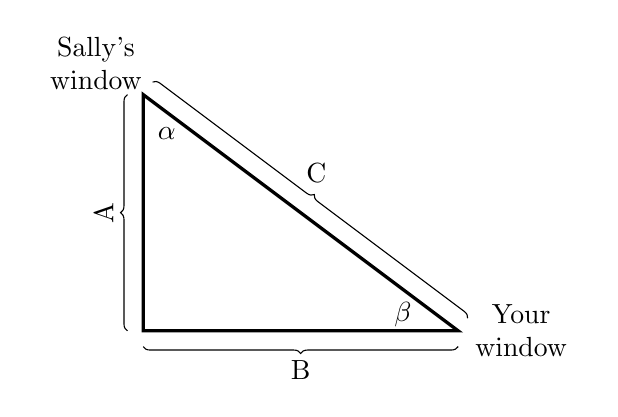
\begin{tikzpicture}
		    \coordinate (C) at (0,2);
		    \coordinate (D) at (0,-1);
		    \coordinate (E) at (4,-1);
		    %\tkzMarkRightAngle(C,D,E)
		    %\tkzMarkAngle(C,E,D)
		    %\tkzMarkAngle(D,C,E)
		    \draw[decoration={brace,mirror, raise=.2cm},decorate,thin] (0,-1)--(4,-1);
		    \draw[decoration={brace,mirror,raise=.2cm},decorate,thin] (0,2)--(0,-1);
		    \draw[decoration={brace, raise=.2cm},decorate,thin] (0,2)--(4,-1);
		    \draw[very thick] (D)--(E)--(C)--cycle;
		    \node at (2,.-1-.5) {B};
		    \node[rotate=90] at (0-.5,.5) {A};
		    \node at (2.2,1) {C};
		    \node at (.3,1.5) {$\alpha$};
		      \node at (3.3,-.8) {$\beta$};
		      \node at (-.6,2.4) {\parbox{1.5cm}{\centering Sally's \\ window}};
		      \node at (4.8,-1) {\parbox{1.5cm}{\centering Your \\ window}};
		  \end{tikzpicture}
		\end{image}

Label all known lengths and angles with units (exact answers in ft and radians):
\begin{enumerate}
\item $A$ is the \wordChoice{\choice{\text{distance across the alley}}\choice[correct]{\text{height difference from Sally's window to yours}}}. We do not know this yet.

\item $B$ is the \wordChoice{\choice[correct]{\text{distance across the alley}}\choice{\text{height difference from Sally's window to yours}}}, which is $\answer{10}$ ft.

\item $\beta$ is the angle between the string and \wordChoice{\choice{\text{Sally's building}}\choice[correct]{\text{your windowsill}}}. \smallskip\\
$\beta = \answer{\frac{5\pi}{12}}$ radians.

\item $\alpha$ is the angle between the string and \wordChoice{\choice[correct]{\text{Sally's building}}\choice{\text{your windowsill}}}. \smallskip\\
$\alpha = \answer{\frac{\pi}{12}}$ radians.
\end{enumerate}

\item How long a piece of string must you cut (give exact value)? $C = \answer{10(\sqrt{6}+\sqrt{2})}$ ft.

\item What is the difference in height between Sally's windowsill and yours? $A = \answer{20+10\sqrt{3}}$ ft.

\item \begin{exercise}
Your friend Sam lives on the second floor of Sally's building, After seeing your set-up, he asks if you can connect a coffee can phone to him too. 
Your buildings are old, so the distance between windowsills may not be the same for each floor of the building. For simplicity, you assume the angle between your windowsill and building is half of angle $\alpha$ above.
% what would be the angles and length of string for you to connect to Sam too?
%
\begin{enumerate}
\item Again, consider a picture of the problem and label all known distances and angles.
\begin{image}[2in]
		  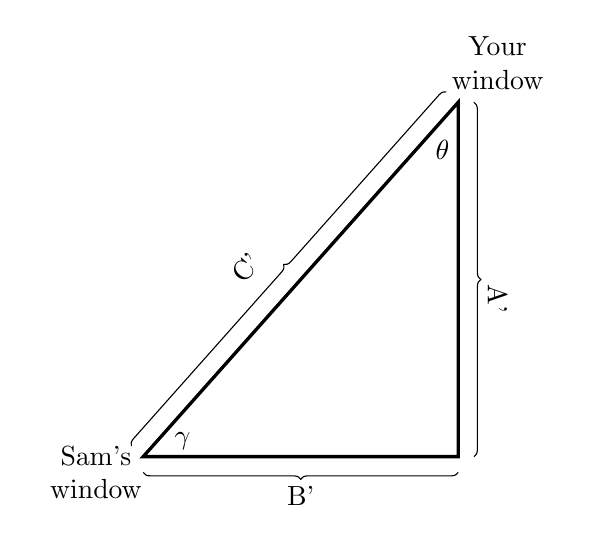
\begin{tikzpicture}
		    \coordinate (C) at (0,2);
		    \coordinate (D) at (4,2);
		    \coordinate (E) at (4,6.5);
		    %\tkzMarkRightAngle(C,D,E)
		    %\tkzMarkAngle(C,E,D)
		    %\tkzMarkAngle(D,C,E)
		    \draw[decoration={brace,mirror,raise=.2cm},decorate,thin] (0,2)--(4,2);
		    \draw[decoration={brace,mirror,raise=.2cm},decorate,thin] (4,2)--(4,6.5);
		    \draw[decoration={brace,raise=.2cm},decorate,thin] (0,2)--(4,6.5);
		    \draw[very thick] (D)--(E)--(C)--cycle;
		    \node at (2,2-.5) {B'};
		    \node[rotate=-90] at (4+.5,4) {A'};
		    \node[rotate=48.5] at (1.4-.1,3.8+.6) {C'};
		    \node at (3.8,5.9) {$\theta$};
		    \node at (.5, 2.2) {$\gamma$};
		     \node at (-.6,1.8) {\parbox{1.5cm}{\centering Sam's \\ window}};
		      \node at (4.5,7) {\parbox{1.5cm}{\centering Your \\ window}};
		  \end{tikzpicture}
		\end{image}

Label all known lengths and angles with units (exact answers):
\begin{enumerate}
\item $\theta$ is the angle between the string and \wordChoice{\choice[correct]{\text{your building}}\choice{\text{Sam's windowsill}}}. \smallskip\\
$\theta = \answer{\frac{\pi}{6}}$ radians.

\item $\gamma$ is the angle between the string and \wordChoice{\choice{\text{your building}}\choice[correct]{\text{Sam's windowsill}}}. \smallskip\\
$\gamma = \answer{\frac{\pi}{3}}$ radians.

\item $B'$ is the \wordChoice{\choice[correct]{\text{distance across the alley}}\choice{\text{height difference from Sam's window to yours}}},  which is $\answer{10}$ ft.

\item $A'$ is the \wordChoice{\choice{\text{distance across the alley}}\choice[correct]{\text{height difference from Sam's window to yours}}}. \smallskip\\
 $A' = \answer{20}$ ft.
\end{enumerate}

\item How long do you have to cut the string to connect a can to Sam's window too?\smallskip\\
 $C' = \answer{20}$ ft.
\end{enumerate}	
\end{exercise}
\end{enumerate}

\end{exercise}
\end{document}
